                %%%%%%%%%%%%%%%%%%%%%%%%%%%%%%%%%%%%%%%%%%%%%%%%%%%%%%%%%%%%%%%%%%%%%%%%%%%%%%%%
%2345678901234567890123456789012345678901234567890123456789012345678901234567890
%        1         2         3         4         5         6         7         8

\documentclass[letterpaper, 10 pt, conference]{ieeeconf}  % Comment this line out
                                                          % if you need a4paper
%\documentclass[a4paper, 10pt, conference]{ieeeconf}      % Use this line for a4
\usepackage{url}
\usepackage[font=footnotesize,labelfont=bf]{caption}
\usepackage{graphicx}
\usepackage[scientific-notation=true]{siunitx}
\usepackage{subcaption}
\usepackage{setspace}
\usepackage[top=0.6 in, bottom=0.7 in, left=0.7in, right=0.7in]{geometry}
\usepackage{blindtext}
\usepackage[utf8]{inputenc}
\usepackage{setspace}
\usepackage{vector}
\usepackage{amsmath}
\usepackage{empheq}
\usepackage{amssymb}
\usepackage{tgtermes}
\usepackage{gensymb}
\DeclareGraphicsExtensions{.pdf,.png,.jpg}
\usepackage{epstopdf}
\usepackage[singlelinecheck=false]{caption}
\usepackage{datetime}
\usepackage[hyperfootnotes=false, pdfnewwindow, colorlinks=true]{hyperref}

\AtBeginDocument{% optionally set colors to your liking
  \hypersetup{
    urlcolor=red,
    citecolor=green,
    linkcolor=blue,
  }%
}                                                         % paper

\IEEEoverridecommandlockouts                              % This command is only
                                                          % needed if you want to
                                                          % use the \thanks command
\overrideIEEEmargins

\title{\LARGE \bf
  On the Commissioning of the 12 GeV HMS Drift Chambers, Electronics/Computer Dead Time Monitoring
  and Overview of the D(e,e'p)n Experimental Run Plan}


\author{Carlos Yero \\
October 30, 2017}

\begin{document}

\twocolumn[
  \begin{@twocolumnfalse}
    \maketitle
    \begin{abstract}
      Three separate topics, all of equal importance, are briefly discussed. The new (12 GeV Era) HMS Drift Chambers are ready to be put in the HMS
      detector stack, in place of the old HMS Chambers. Several efficcinecy tests were performed on one of the chambers during the second week of October
      2017. The efficciecies were determined to be better than 99$\%$. The second chamber has not been tested yet, but it is
      expected to behave the same since both chambers were tested under similar conditions in the past. Dead time studies are currently in progress to
      determine how many physics events (triggers) are actually lost due to computer and electronic deadtime inherent in our experimental equipment. 
      There had been some technical issues found related to the computer livetime that are being addressed by the Jefferson Lab DAQ group. The experimental run
      plan of my thesis experiment, the electro-disintegration of Deuteron, is briefly discussed as the kinematics have slightly changed and new
      simulations had to be done. \\      
    \end{abstract}
  \end{@twocolumnfalse}
  ]

%%%%%%%%%%%%%%%%%%%%%%%%%%%%%%%%%%%%%%%%%%%%%%%%%%%%%%%%%%%%%%%%%%%%%%%%%%%%%%%


  

%%%%%%%%%%%%%%%%%%%%%%%%%%%%%%%%%%%%%%%%%%%%%%%%%%%%%%%%%%%%%%%%%%%%%%%%%%%%%%%%
\section{INTRODUCTION}
On March 7-10 of 2017, a 5 $\mu$A electron beam was delivered to a BeO and Carbon targets for the first time to experimental
Hall C since the 12 GeV upgrade. The beam was delivered as part of the Key Performance Parameters (KPP) required by the
Department of Energy (DOE) to demonstrate the operability of the High Momentum Spectrometer (HMS) and Super HMS (SHMS). 
Hall C was able to demonstrate KPP in four days of beam time before an important component of the accelerator was damaged which
caused to accelerator to shut down for repair. The accelerator is expected to be operational starting December 4, 2017. As a
result of this delay, the commissioning experiments that were scheduled to run on Fall 2017 have now shifted to Spring 2018.
This time window has allowed the Hall C collaboration to work extensively in preparation for the commissioning of the
spectrometers on December. \\
\indent One of the projects I have been involved in is the ongoing work on testing and commissioning the 12 GeV HMS Drift
Chambers. The chambers were constructed at Hampton University by Dr. Liguang Tang and his graduate students in 2016.
They were made the same design as the SHMS chambers, but slightly different size. The chambers were transported to Jefferson Lab on November 2016,
where they underwent extensive tests as part of conditioning the chambers to sustain High Voltages using a gas mixture\footnote{This gas mixture is non-flammable and
at lower cost compared to the gas mixture that the chambers run on during an experiment, which is why it is preferred during the testing phase of the detector.}
of 75:25 Argon/CO$_{2}$ by volume. The chambers were found to be operational below 1850 V which is below the expected value\footnote{The HMS chambers
are the same design as the SHMS chambers, which operate at $\sim$ 1940 V.} of 1940 V. At high voltages above 1850 V, the chambers drew a significant amount of
dark current which made the signals from the chamber noisy.
It was determined that the most likely cause of the large currents drawn was the gas mixture[Ar/CO$_{2}$] being used, so the one of the chambers (HMS DC II) was transported to the
experimental Hall C where a gas mixture of 50:50 Argon/Ethane by volume was used. A test stand for the chamber was set up in the HMS hut, where it has been tested and
verified to be operational with the new gas mixture. The other chamber (HMS DC I) exhibited similar symptoms as the first with the addition that it had a few missing channels
due to a bad connection between the sense wires and the discriminator cards. The second chamber is now ready to be transported to Hall C for further tests with the
Argon/Ethane gas mixture before it can be put in the detector stack.\\
\indent A second project I am currently involved in is the determination of electronic and computer dead times. In nuclear/particle physics experiments,
the number of physics events (triggers) are counted via nuclear electronic modules. These triggers ultimately get processed by the DAQ before being
written to tape. The deadtime refers to the time window in which the modules are unable to process triggers and physics events are lost.
The electronic deadtime contribution comes from the electronic modules having a maximum rate capability. Typically,
the electronic modules in Hall C can achieve rates from a few MHz to few hundred MHz. Once the modules reach their limit, a pileup of signals can occur which
contributes to the total dead time. The computer deadtime contribution comes from finite processing time of the DAQ. These rates are typically on the order of
a few kHz, therefore, the dominant contribution of total dead time comes from the DAQ, since it takes a few kHz of data before physics events
are lost. These measurements are important for the determination of high precision cross section measurements in Hall C, since knowing how many events
are actually lost can make a significant difference in the uncertainty of the cross section. \\
\indent My thesis experiment, the \textit{Electro-Disintegration of Deuteron at Very High Missing Momenta} is projected to run towards the end of
February 2018, and will receive a total of six days of beam time. The experiment will be done at four different spectrometer configurations. The kinematic
setting have changed slightly from the original proposal, and will be briefly discussed in this paper. 


\section{12 GeV HMS Drift Chambers}


\subsection{Design and Operation of the Chambers}
The new HMS Drift Chambers were designed to be geometrically the same as the SHMS Drift Chambers. Each chamber consists of 6 wire planes and each wire
plane is located between two cathode planes. The wire planes consist of alternating field and sense wires. The U, U', V and V' planes consist of
96 sense wires each and are oriented 60$^{o}$ relative to the +y-coordinate. The X and X' planes consist of 102 sense wires and are oriented perpendicular to the x-axis (See
Figures \ref{fig:dc1_planes} and \ref{fig:dc_wires}).
\begin{figure}[h!]
  \centering
  \includegraphics[width=3.0in, height=2.5in]{dc2_tests/HMS_DC1_Planes.pdf}
  \caption{HMS Drift Chamber 1 wire planes.}
  \label{fig:dc1_planes}
\end{figure}
\begin{figure}[h!]
  \centering
  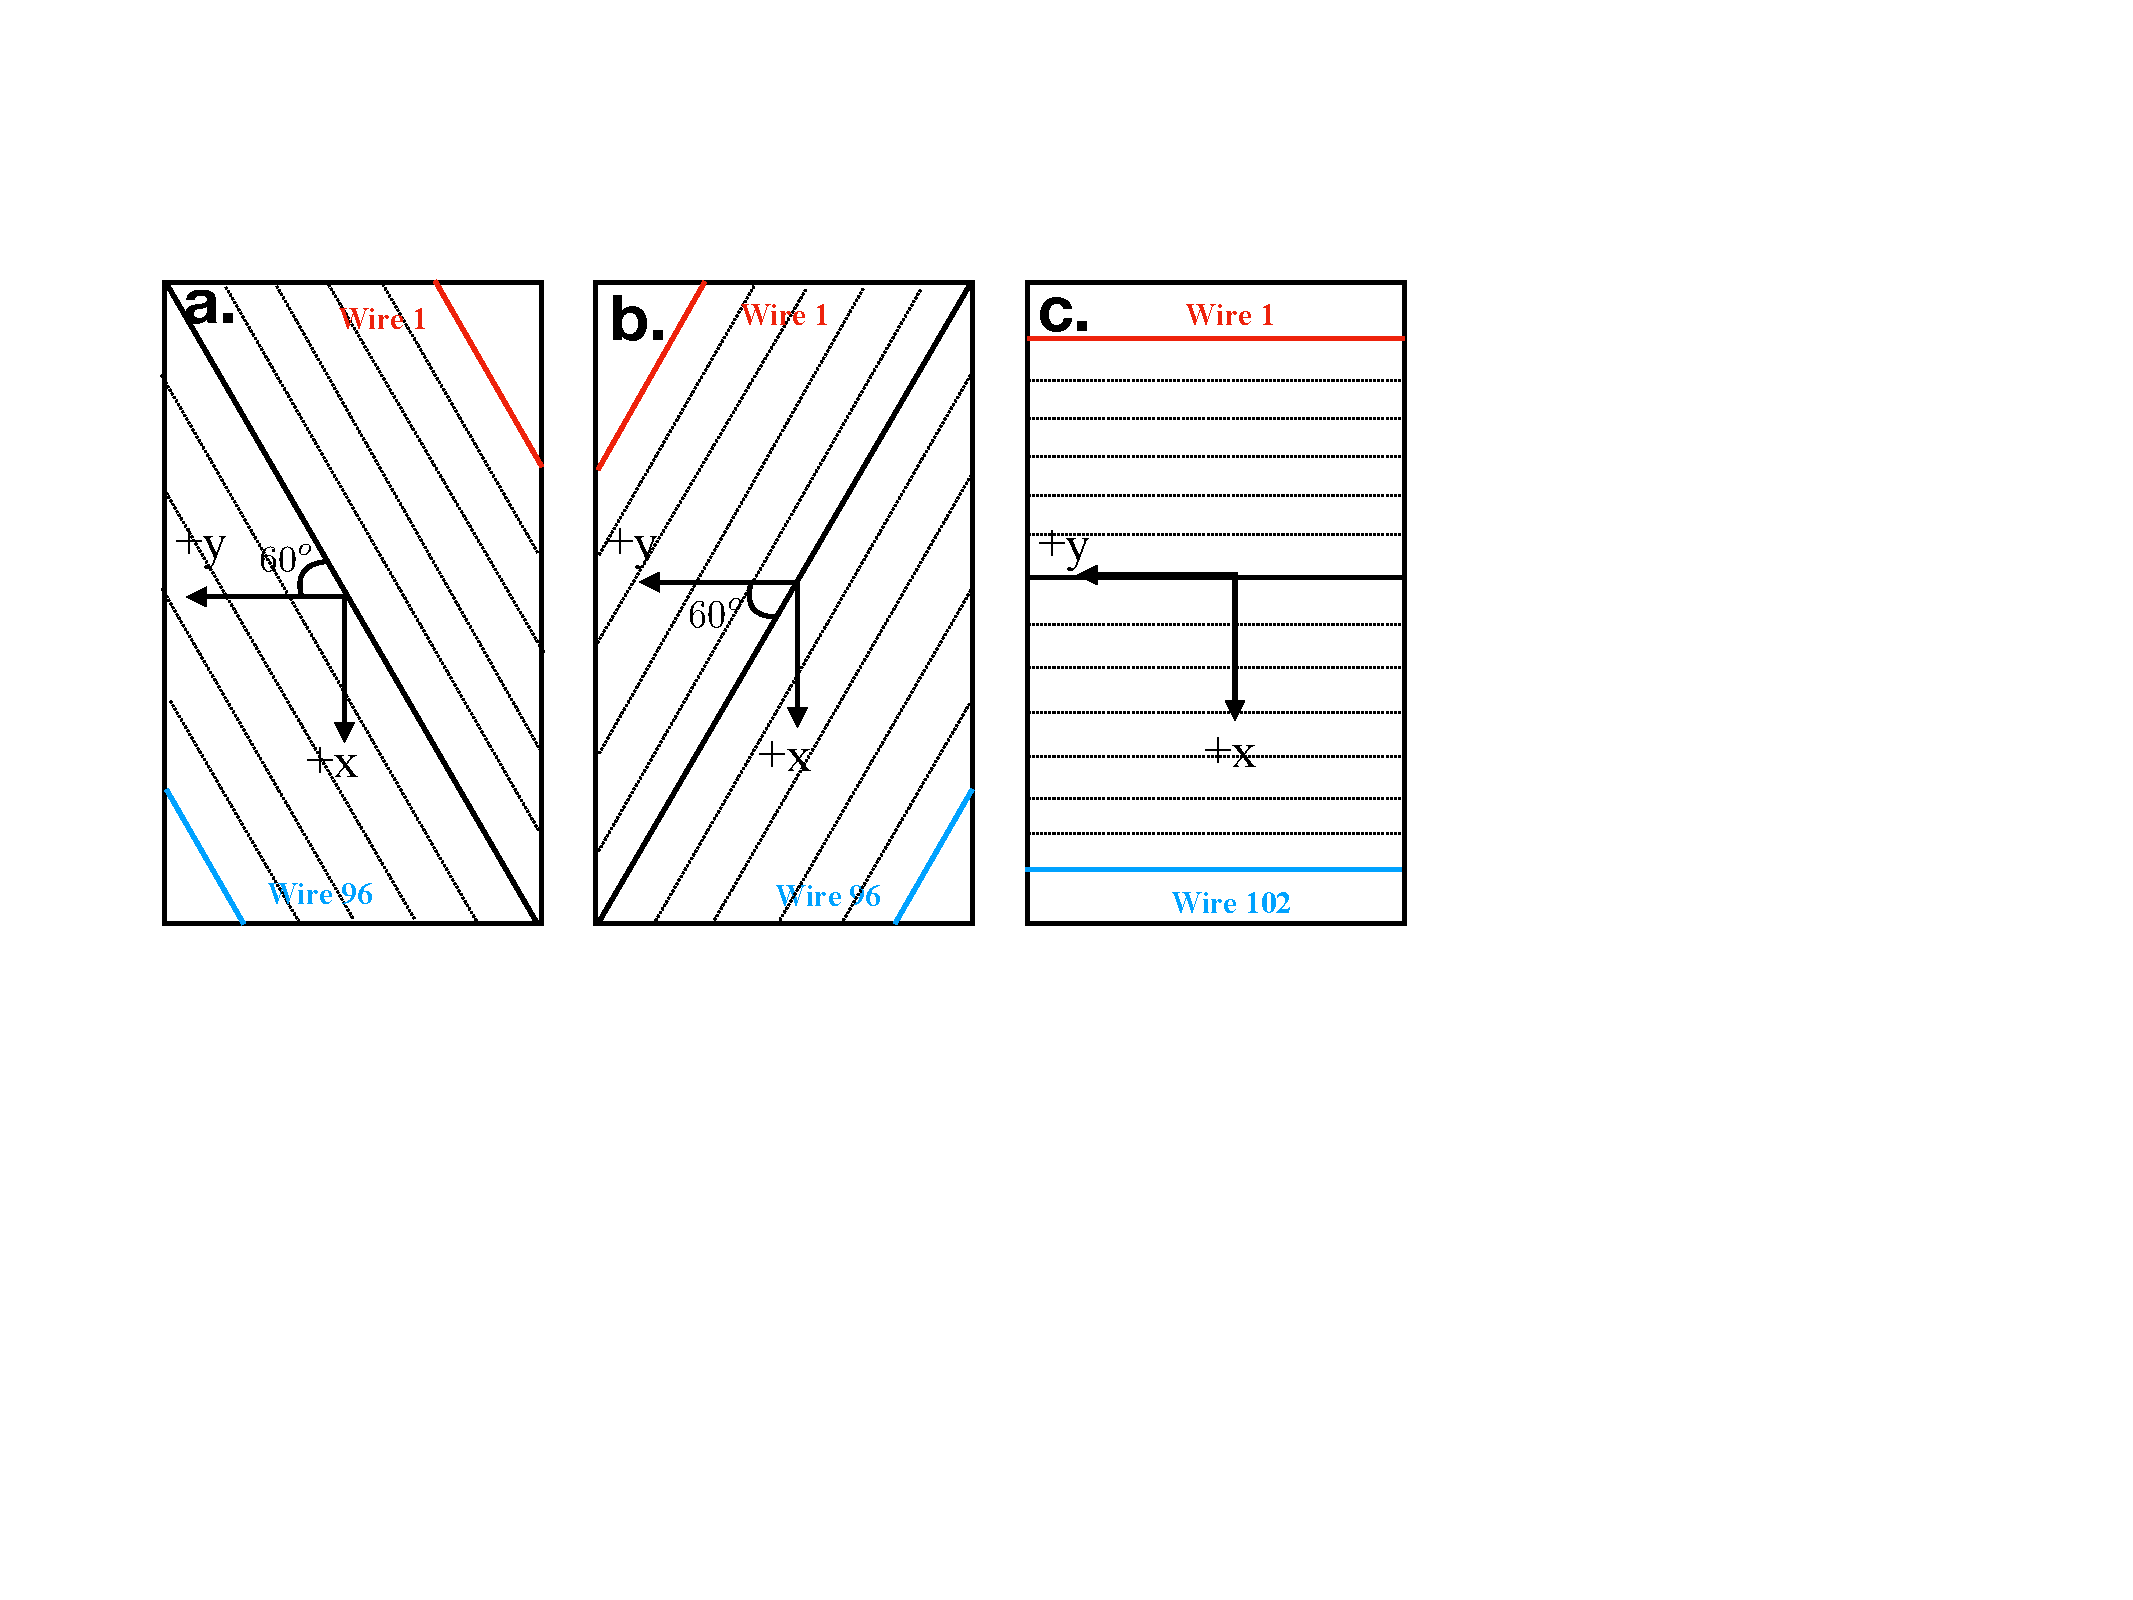
\includegraphics[width=3.0in, height=1.5in]{dc2_tests/HMS_DC_Wires.pdf}
  \caption{HMS Drift Chamber wire orientation for planes a) U, U', b) V, V' and c) X, X' where
  the direction of the beam (+z) is into the plane of the paper.}
  \label{fig:dc_wires}
\end{figure}
The cathode planes and field wires are held at a negative high voltage and the sense wires are grounded which establihses a potential gradient causing an electric field
between high voltage and grounded wires. Each chamber is filled with a gas mixture\footnote{Argon is mixed with CO$_{2}$ or Ethane, where Argon is the ionizing agent the
particles interact with, and Ethane/CO$_{2}$ are the quenching elements to control avalanche produced by secondary ionization} of Argon with either CO$_{2}$ or Ethane.
As the particles traverse the chamber, the free electrons from ionized Argon drift towards the sense wires producing a detectable signal which is read out via discriminator
cards and into electronic modules.

\subsection{HMS Drift Chamber Cosmic Tests}
To determine the operatility of the HMS Drift Chambers, several cosmic tests were performed on the chambers in the Experimental Storage Building (ESB) before being transported
to Hall C. The chambers did not held the High Voltage beyond 1850 V without drawing a significant amount of current ($\geq$ 10 $\mu$A ) using a gas mixture of 75:25 Ar/CO$_{2}$ by
volume. When Drift Chamber II (DCII) was transported to Hall C, the gas mixture was changed to 50:50 Ar/Ethane and a High Voltage scan was done (See Figure \ref{fig:current_draw})  
\begin{figure}[h!]
  \centering
  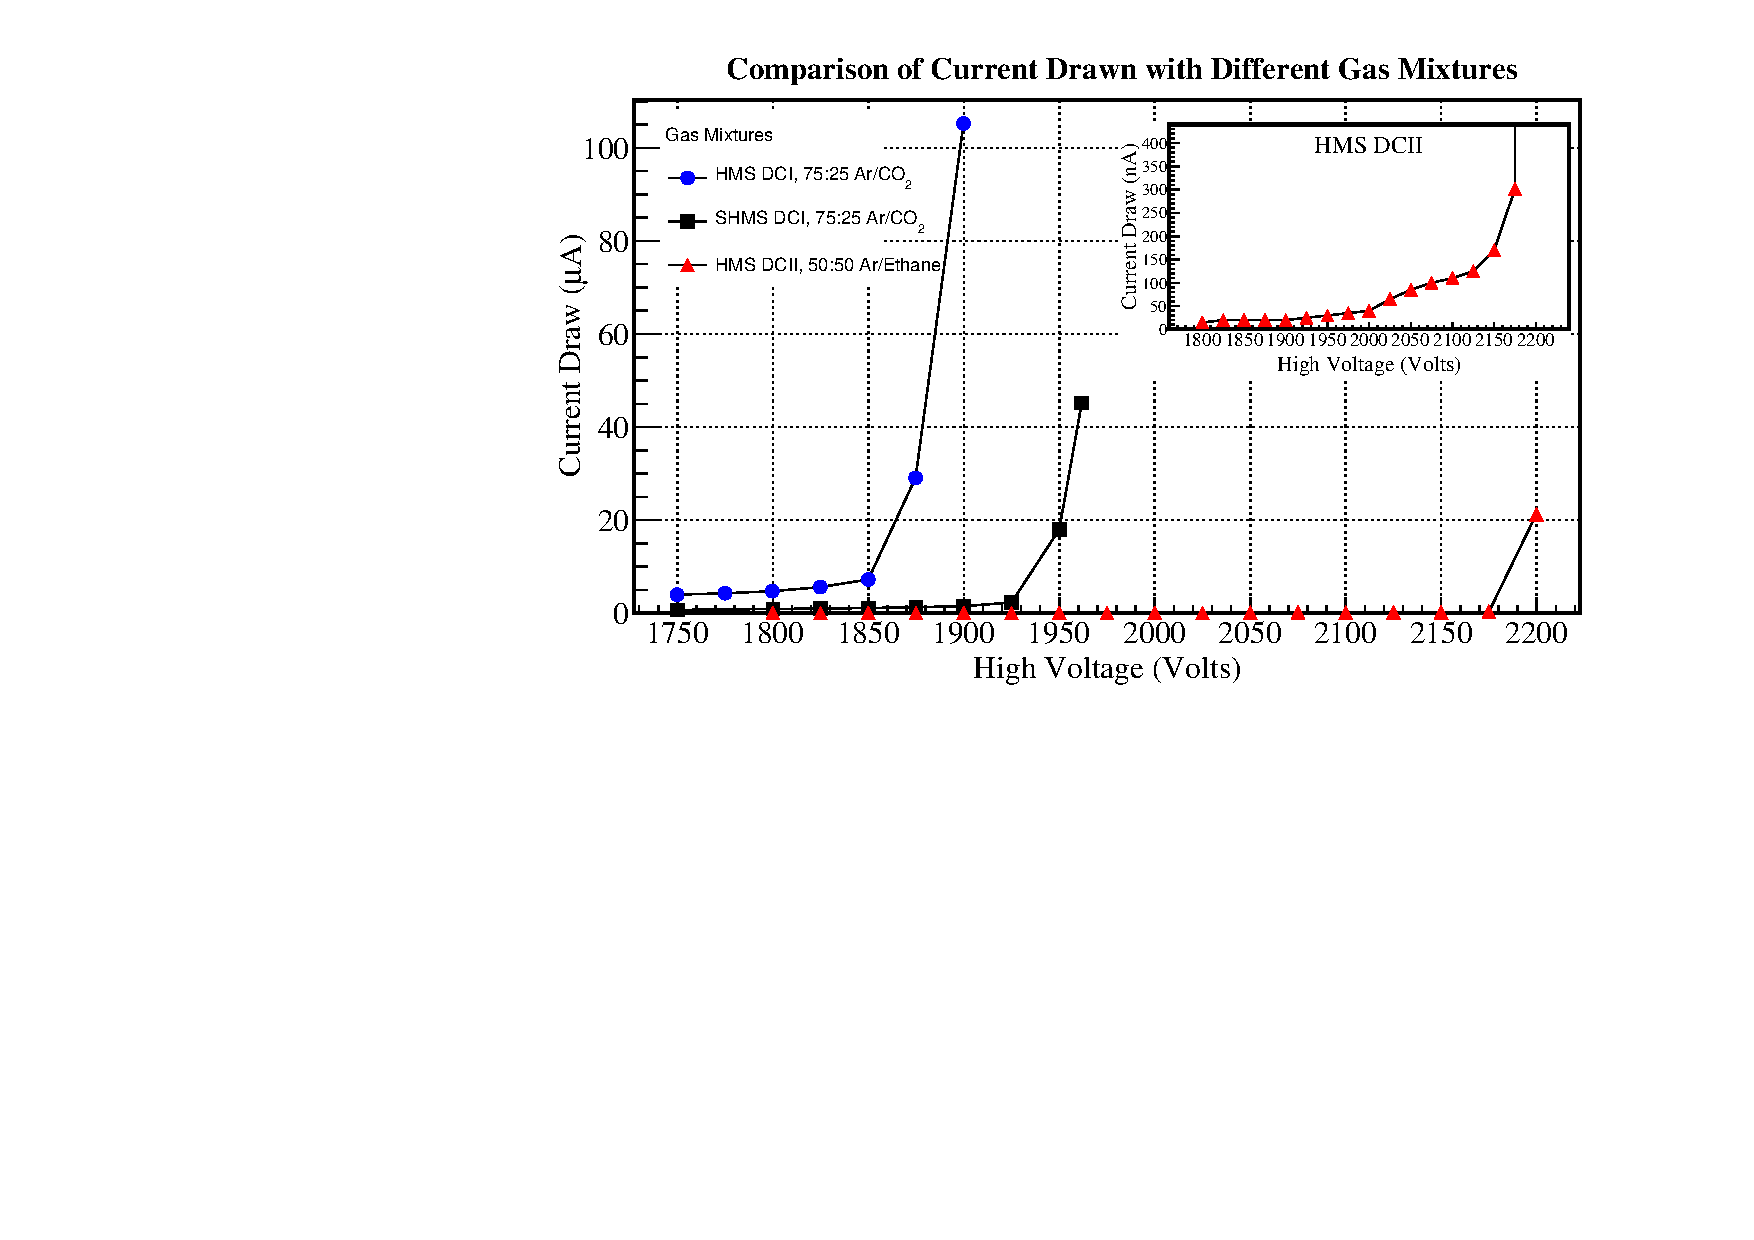
\includegraphics[width=4.0in, height=2.4in]{dc2_tests/gas_mix_current_drawn.pdf}
  \caption{Comparison of the current drawn in the HMS and SHMS chambers for different gas mixtures. The subplot shows a zoomed version of the Argon/Ethane gas mixture used in HMS DC II plot on a nanoampere scale.}
  \label{fig:current_draw}
\end{figure} \\
Figure \ref{fig:current_draw} shows a decrease is the current drawn by the HMS chambers by three orders of magnitude smaller, from a few $\mu$A to a few nA of current drawn. This
indicates that Ethane is a better quenching gas, as it kept the secondary electron ionization small for a broader range of High Voltages, up to $\sim$2100 Volts. There is still the
unresolved issue of why the HMS and SHMS chambers behave differently with the same gas mixture, since they both have the same design. The broad High Voltage range achieved by DC II without
significant current drawn allows for a better determination of the \textit{Plateau Region} of the chambers, which is a region in which the chamber efficiencies have little sensitivity
to relatively large High Voltage variations. \\
\indent To determine the plateau region of HMS DC II,  a cosmic test stand was set up in the HMS detector hut (See Figure \ref{fig:cosmic_stand}). The setup consists of two scintillator paddles on the top
and two on bottom of the chamber. The top two are completely overlapped while the bottom two are only partially overlapped. Each scintillator paddle is wrapped around a light tight material known as Tedlar,
and is coupled to a Photomultiplier Tube (PMT) via a light guide. To ensure that only cosmic rays pass through the chamber, a coincidence between the top and bottom PMTs is made. It is required that the top
two PMTs detect a signal to reduce the probability of instrinsic noise being interpreted as a cosmic signal. The bottom scintillators are partially overlapped to achieve full coverage of the chamber active
area, and a less restrictive requirement was made by requiring that either of the bottom PMTs detect a signal. A final requirement was made so that the top and bottom PMTs would detect a signal within a
certain time window. This requirement ensures a correlation between the top and bottom PMT signals, making it highly probable that the signal was produced by a cosmic ray. The correlated signal between the top and
bottom PMTs is defined as the \textit{trigger}. The efficiency of the \textit{i$^{th}$} plane, $\epsilon_{i}$, can then be defined as follows,
\begin{equation}
\epsilon_{i} = \frac{\# \text{ triggers that \textit{did} hit the \textit{i$^{th}$} plane } }{\# \text{ triggers that \textit{should} have hit the \textit{i$^{th}$} plane} } 
\end{equation}
given that the other five planes received at least one hit from the cosmic. \\
\indent To make a reliable efficiency measurement, it has to be ensured from the geometry of the cosmic set-up, that any cosmic passing though the top and bottom scintillators also traverses every plane in the chamber
to make the efficiency measurements unbiased to the scintllators orientation. 
\begin{figure}[h!]
  \centering
  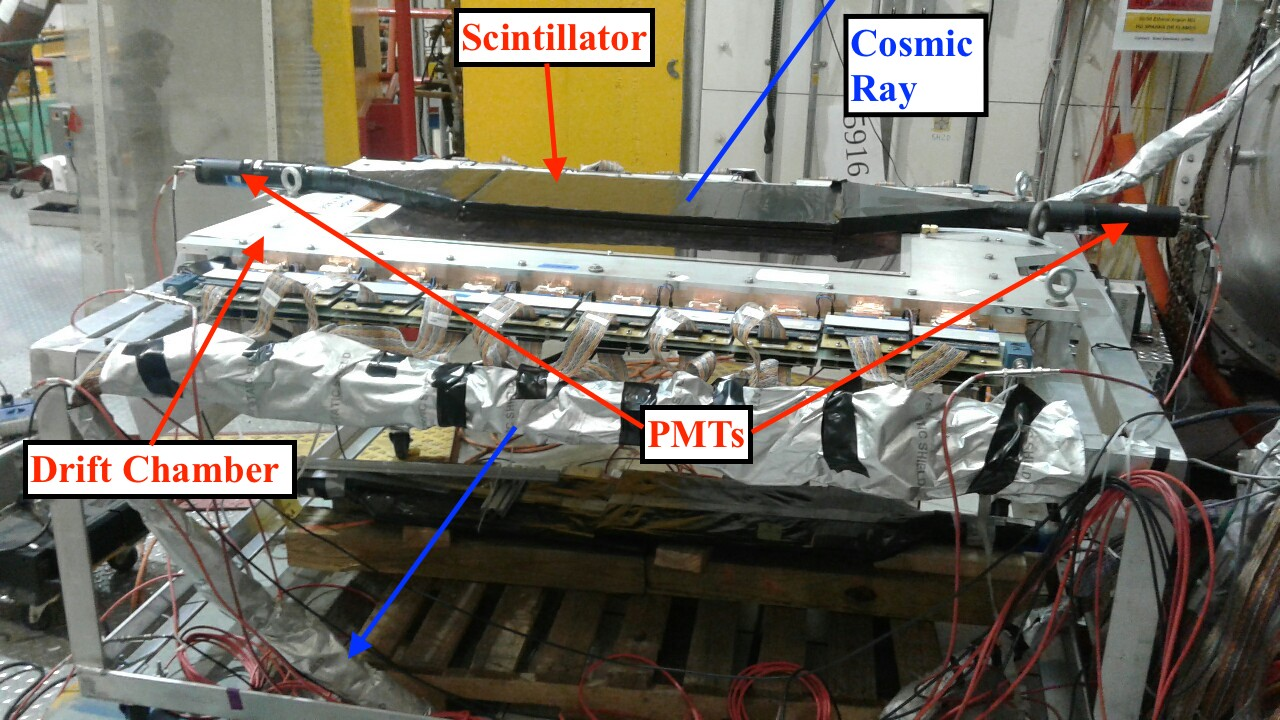
\includegraphics[width=3.4in, height=2.4in]{dc2_tests/dc2_teststand_03.jpg}
  \caption{Cosmic test stand setup in Hall C detector hut.}
  \label{fig:cosmic_stand}
\end{figure} \\
When cosmic data was taken, to ensure that all (or at least most) of the sense wires in each plane were present (and had not been damaged by transporting the chamber), the wiremap distribution was
a looked at first. The distributions show full occupancy for all wire planes in DC II (See Figure \ref{fig:hdc2_wiremap}).  
\begin{figure}[h!]
  \centering
  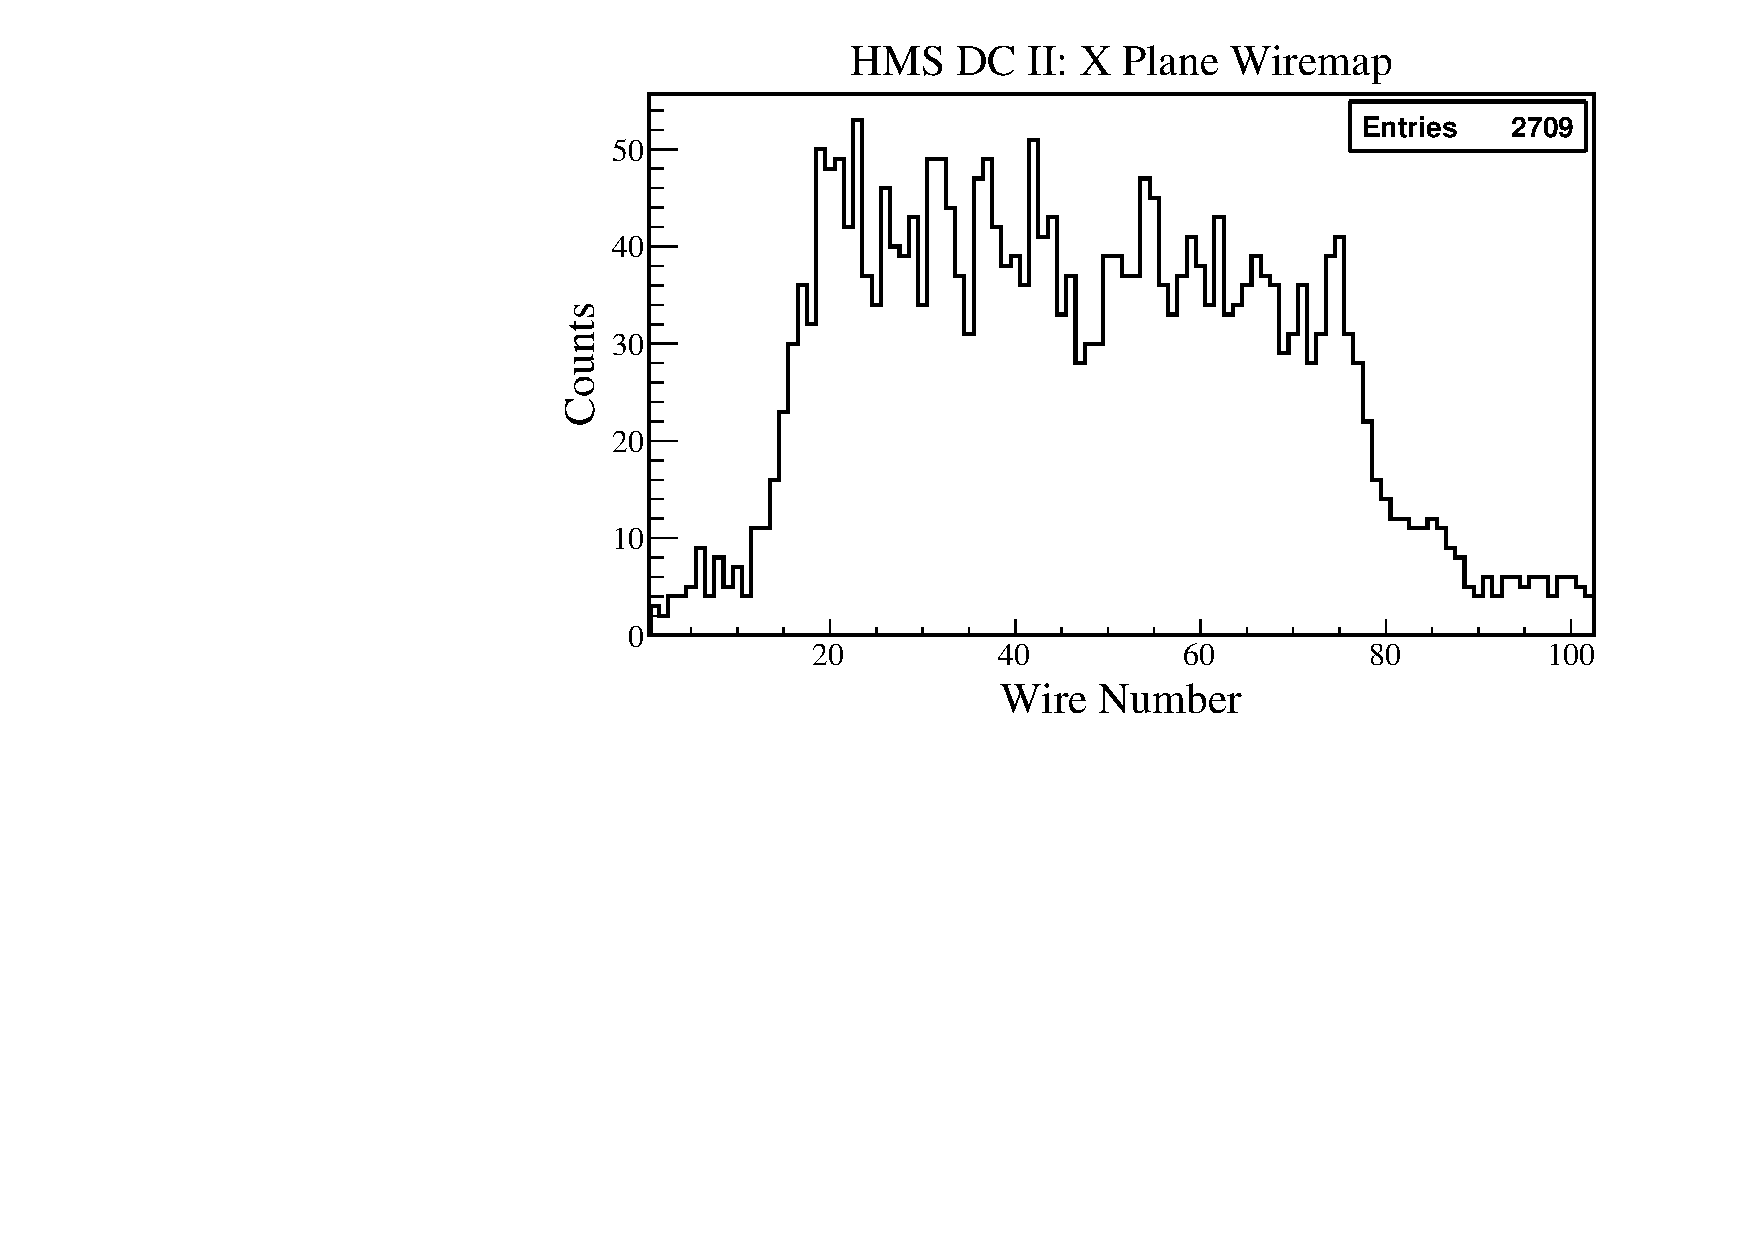
\includegraphics[width=3.8in, height=2.2in]{dc2_tests/hdc2_xmap.pdf}
  \caption{Wiremap distribution of the X Plane in DC II shows occupancy in all wires.}
  \label{fig:hdc2_wiremap}
\end{figure} \\
Once all planes of the chamber were verified to have full occupancy, a High Voltage and threshold\footnote{The threshold set on the chamber is used to filter cosmic signals from noise by requiring 
the signal amplitude to cross a threshold before discriminating them to produce logic signals, which are read out by the electronic modules.} scan was done to determine the plateau region. A high voltage scan was done first
by setting the threshold fixed at 4.5 V to determine the optimal HV setting. A threshold scan was then performed at 1940 V to determine the optimal threshold. The results are shown in Figures \ref{fig:hdc2_hvscan}
and \ref{fig:hdc2_thrsscan}. The high voltage scan in Figure \ref{fig:hdc2_hvscan} shows the plateau region starting at 1900 V. The chamber operational high voltage was chosen to be 1940 V since the efficiencies seem
to be stable and better than 99$\%$ over a $\sim\pm$40 Volt range about this central setting.
\begin{figure}[h!]
  \centering
  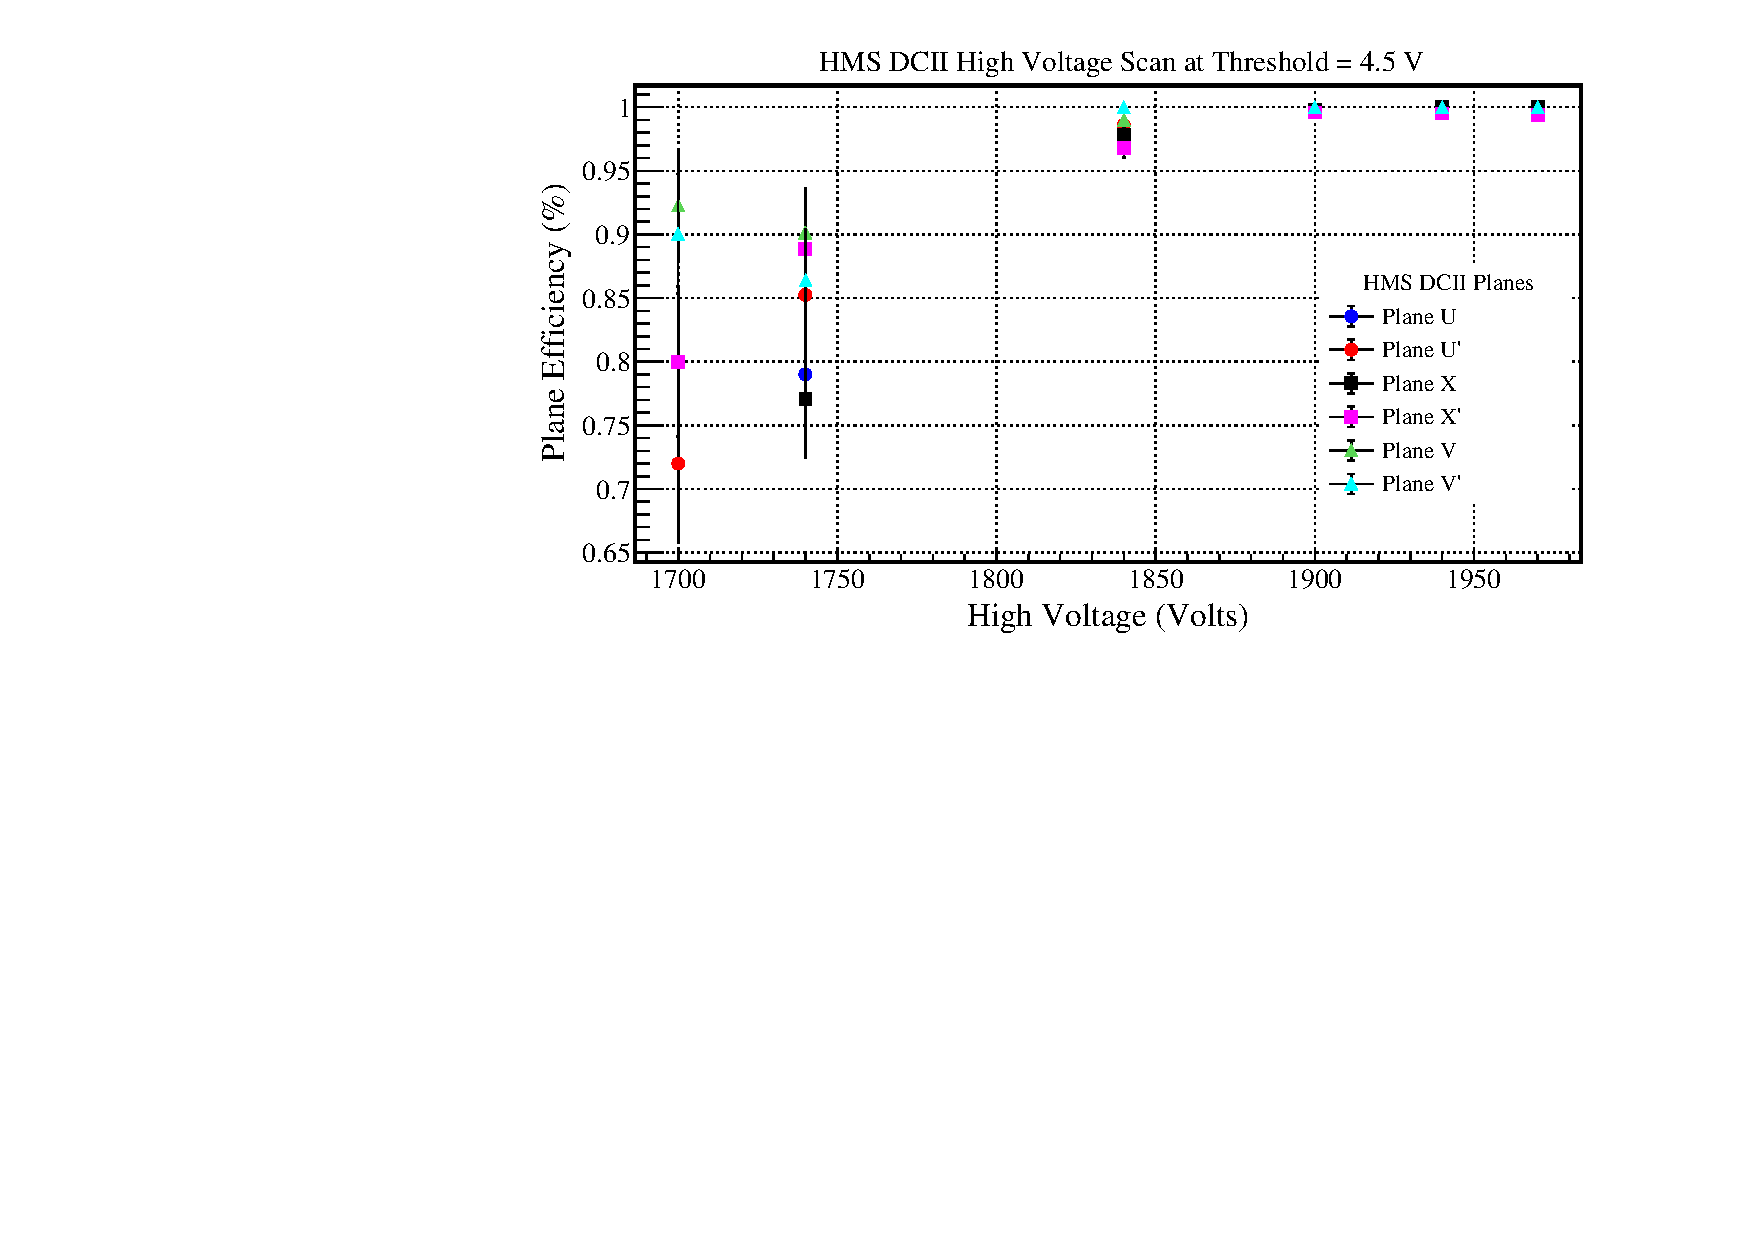
\includegraphics[width=4.1in, height=2.2in]{dc2_tests/dc2_hvscan_thrs45.pdf}
  \caption{High Voltage scan of DC II over a broad range at a Threshold of 4.5 Volts.}
  \label{fig:hdc2_hvscan}
\end{figure} 
\begin{figure}[h!]
  \centering
  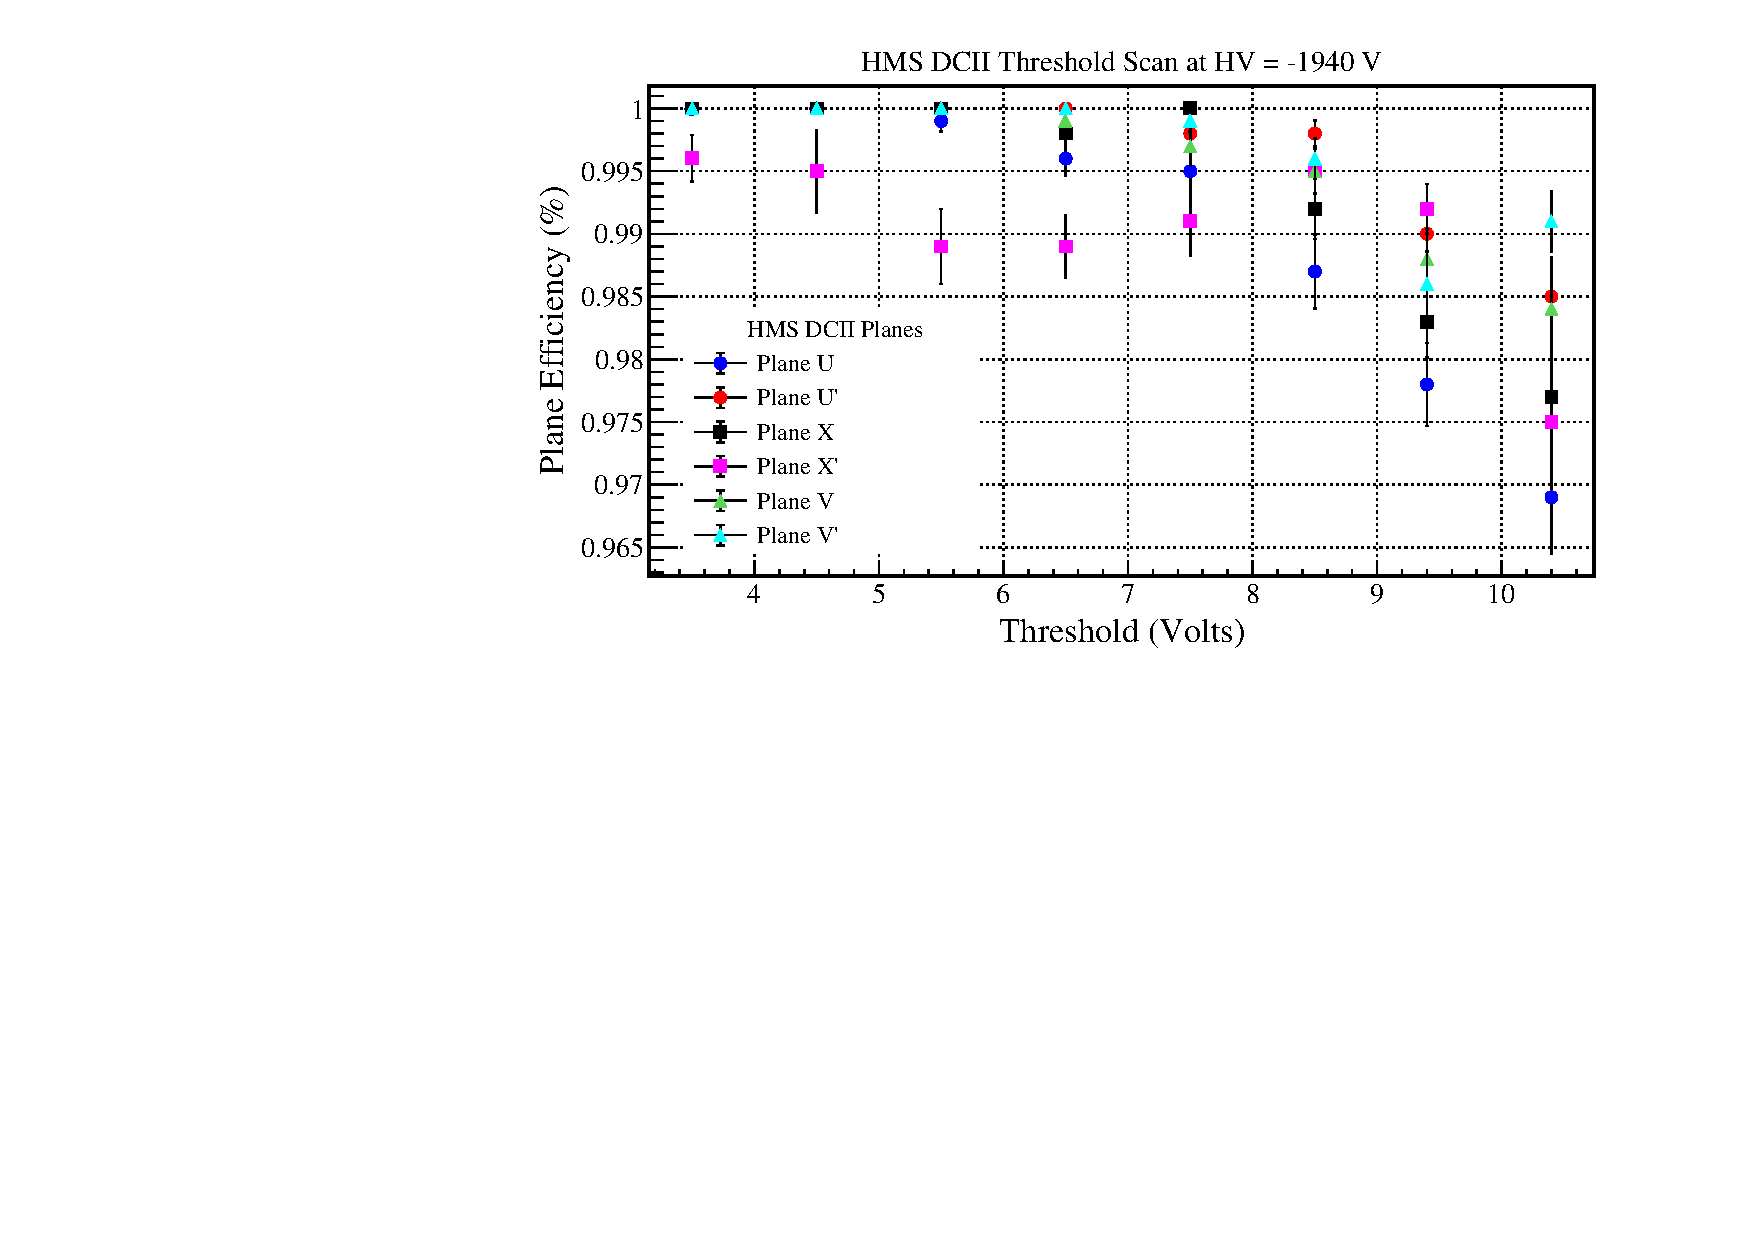
\includegraphics[width=4.1in, height=2.2in]{dc2_tests/dc2_thrsscan_HV_1940V.pdf}
  \caption{Threshold scan over a broad range at a HV setting of 1940 V.}
  \label{fig:hdc2_thrsscan}
\end{figure} \\
From the threshold scan results in Figure \ref{fig:hdc2_thrsscan}, there is a 3$\%$ decrease in the plane efficiencies over a
6 Volt range. The operational threshold voltage was determined to be 4.5 Volts, where the efficiencies are better than 99$\%$, over a $\sim$ 1 Volt range.
The high voltage and threshold settings determined from the scans were chosen based on the high efficiency region and its small sensitivity over a voltage range.  


\section{Electronic and Computer Deadtime Studies}
The procedure to determine the computer and electronic dead times is currently in the development stage in Hall C. The general idea is to use a pulse generator to produce
a fixed frequency pulse and feed it as early as possible into the electronic modules being used in the experimental setup. This pulse will interfere wth the actual signals
produced by physics, but its rate can be set orders of magnitude smaller such that its interference will be minimal and will have insignificant contribution to the deadtime.
By counting the number of pulses generated before sending them to the electronics chain, compared to the number of pulses that actually make it to the end of the chain and
are accepted by the TI (Trigger Interface) module, one may determine the dead time as follows:
\begin{equation}
  \text{dead time} = 1 - \frac{\# \text{ of accepted pulses}}{\# \text{ of generated pulses}}
\end{equation}
This is the total deadtime from the electronics and computer (TI module) that arises due to the finite processing time of the modules. The computer live time alone is calculated by the TI module since it has an
internal scaler which counts the number of input and output signals, and takes the ratio to determine the computer live time. This calculation can also be done externally as a cross-check by counting the number of signals that make it to the
TI via a scaler module, and comparing it to the number of accepted signals which is outputted by the TI and determined during the data analysis stage. The electronics deadtime is investigated by keeping the computer live time near 100$\%$ and
increasing the pulse generator rate to probe the rate limits of the electronics modules. One might argue that such high rates can reduce the computer live time itself which is true, however, such high rates can be pre-scaled by the TI by orders
of magnitude, such that the computer live time is preserved. For example, for every 10,000 counts/sec., (10 KHz), the TI counts 100 Hz., so that the rate is pre-scaled by a factor of 10$^{3}$. Using this technique, one can investigate the
effects of high rates on the electronic modules. In this limitng case, the total live time measured will be the electronics live time, since the computer live time will be fixed. \\
\indent The electronic and computer live time measurements have not been completed as there had been some issues encountered with the TI module that is currently being investgated by DAQ experts. These issues were uncovered during the
initial stages of the deadtime studies in which a pulse generator at various rates was used to probe the limits of the modules. 

Before you begin to format your paper, first write and save the content as a separate text file. Keep your text and graphic files separate until after the text has been formatted and styled. Do not use hard tabs, and limit use of hard returns to only one return at the end of a paragraph. Do not add any kind of pagination anywhere in the paper. Do not number text heads-the template will do that for you.

Finally, complete content and organizational editing before formatting. Please take note of the following items when proofreading spelling and grammar:

\subsection{Abbreviations and Acronyms} Define abbreviations and acronyms the first time they are used in the text, even after they have been defined in the abstract. Abbreviations such as IEEE, SI, MKS, CGS, sc, dc, and rms do not have to be defined. Do not use abbreviations in the title or heads unless they are unavoidable.

\subsection{Units}

\begin{itemize}

\item Use either SI (MKS) or CGS as primary units. (SI units are encouraged.) English units may be used as secondary units (in parentheses). An exception would be the use of English units as identifiers in trade, such as Ò3.5-inch disk driveÓ.
\item Avoid combining SI and CGS units, such as current in amperes and magnetic field in oersteds. This often leads to confusion because equations do not balance dimensionally. If you must use mixed units, clearly state the units for each quantity that you use in an equation.
\item Do not mix complete spellings and abbreviations of units: ÒWb/m2Ó or Òwebers per square meterÓ, not Òwebers/m2Ó.  Spell out units when they appear in text: Ò. . . a few henriesÓ, not Ò. . . a few HÓ.
\item Use a zero before decimal points: Ò0.25Ó, not Ò.25Ó. Use Òcm3Ó, not ÒccÓ. (bullet list)

\end{itemize}


\subsection{Equations}

The equations are an exception to the prescribed specifications of this template. You will need to determine whether or not your equation should be typed using either the Times New Roman or the Symbol font (please no other font). To create multileveled equations, it may be necessary to treat the equation as a graphic and insert it into the text after your paper is styled. Number equations consecutively. Equation numbers, within parentheses, are to position flush right, as in (1), using a right tab stop. To make your equations more compact, you may use the solidus ( / ), the exp function, or appropriate exponents. Italicize Roman symbols for quantities and variables, but not Greek symbols. Use a long dash rather than a hyphen for a minus sign. Punctuate equations with commas or periods when they are part of a sentence, as in

$$
\alpha + \beta = \chi \eqno{(1)}
$$

Note that the equation is centered using a center tab stop. Be sure that the symbols in your equation have been defined before or immediately following the equation. Use Ò(1)Ó, not ÒEq. (1)Ó or Òequation (1)Ó, except at the beginning of a sentence: ÒEquation (1) is . . .Ó

\subsection{Some Common Mistakes}
\begin{itemize}


\item The word ÒdataÓ is plural, not singular. \cite{Leo}
\item The subscript for the permeability of vacuum ?0, and other common scientific constants, is zero with subscript formatting, not a lowercase letter ÒoÓ.
\item In American English, commas, semi-/colons, periods, question and exclamation marks are located within quotation marks only when a complete thought or name is cited, such as a title or full quotation. When quotation marks are used, instead of a bold or italic typeface, to highlight a word or phrase, punctuation should appear outside of the quotation marks. A parenthetical phrase or statement at the end of a sentence is punctuated outside of the closing parenthesis (like this). (A parenthetical sentence is punctuated within the parentheses.)
\item A graph within a graph is an ÒinsetÓ, not an ÒinsertÓ. The word alternatively is preferred to the word ÒalternatelyÓ (unless you really mean something that alternates).
\item Do not use the word ÒessentiallyÓ to mean ÒapproximatelyÓ or ÒeffectivelyÓ.
\item In your paper title, if the words Òthat usesÓ can accurately replace the word ÒusingÓ, capitalize the ÒuÓ; if not, keep using lower-cased.
\item Be aware of the different meanings of the homophones ÒaffectÓ and ÒeffectÓ, ÒcomplementÓ and ÒcomplimentÓ, ÒdiscreetÓ and ÒdiscreteÓ, ÒprincipalÓ and ÒprincipleÓ.
\item Do not confuse ÒimplyÓ and ÒinferÓ.
\item The prefix ÒnonÓ is not a word; it should be joined to the word it modifies, usually without a hyphen.
\item There is no period after the ÒetÓ in the Latin abbreviation Òet al.Ó.
\item The abbreviation Òi.e.Ó means Òthat isÓ, and the abbreviation Òe.g.Ó means Òfor exampleÓ.

\end{itemize}


\section{USING THE TEMPLATE}

Use this sample document as your LaTeX source file to create your document. Save this file as {\bf root.tex}. You have to make sure to use the cls file that came with this distribution. If you use a different style file, you cannot expect to get required margins. Note also that when you are creating your out PDF file, the source file is only part of the equation. {\it Your \TeX\ $\rightarrow$ PDF filter determines the output file size. Even if you make all the specifications to output a letter file in the source - if you filter is set to produce A4, you will only get A4 output. }

It is impossible to account for all possible situation, one would encounter using \TeX. If you are using multiple \TeX\ files you must make sure that the ``MAIN`` source file is called root.tex - this is particularly important if your conference is using PaperPlaza's built in \TeX\ to PDF conversion tool.

\subsection{Headings, etc}

Text heads organize the topics on a relational, hierarchical basis. For example, the paper title is the primary text head because all subsequent material relates and elaborates on this one topic. If there are two or more sub-topics, the next level head (uppercase Roman numerals) should be used and, conversely, if there are not at least two sub-topics, then no subheads should be introduced. Styles named ÒHeading 1Ó, ÒHeading 2Ó, ÒHeading 3Ó, and ÒHeading 4Ó are prescribed.

\subsection{Figures and Tables}

Positioning Figures and Tables: Place figures and tables at the top and bottom of columns. Avoid placing them in the middle of columns. Large figures and tables may span across both columns. Figure captions should be below the figures; table heads should appear above the tables. Insert figures and tables after they are cited in the text. Use the abbreviation ÒFig. 1Ó, even at the beginning of a sentence.

\begin{table}[h]
\caption{An Example of a Table}
\label{table_example}
\begin{center}
\begin{tabular}{|c||c|}
\hline
One & Two\\
\hline
Three & Four\\
\hline
\end{tabular}
\end{center}
\end{table}


   \begin{figure}[thpb]
      \centering
      \framebox{\parbox{3in}{We suggest that you use a text box to insert a graphic (which is ideally a 300 dpi TIFF or EPS file, with all fonts embedded) because, in an document, this method is somewhat more stable than directly inserting a picture.
}}
      %\includegraphics[scale=1.0]{figurefile}
      \caption{Inductance of oscillation winding on amorphous
       magnetic core versus DC bias magnetic field}
      \label{figurelabel}
   \end{figure}
   

Figure Labels: Use 8 point Times New Roman for Figure labels. Use words rather than symbols or abbreviations when writing Figure axis labels to avoid confusing the reader. As an example, write the quantity ÒMagnetizationÓ, or ÒMagnetization, MÓ, not just ÒMÓ. If including units in the label, present them within parentheses. Do not label axes only with units. In the example, write ÒMagnetization (A/m)Ó or ÒMagnetization {A[m(1)]}Ó, not just ÒA/mÓ. Do not label axes with a ratio of quantities and units. For example, write ÒTemperature (K)Ó, not ÒTemperature/K.Ó

\section{CONCLUSIONS}

A conclusion section is not required. Although a conclusion may review the main points of the paper, do not replicate the abstract as the conclusion. A conclusion might elaborate on the importance of the work or suggest applications and extensions. 

\addtolength{\textheight}{-12cm}   % This command serves to balance the column lengths
                                  % on the last page of the document manually. It shortens
                                  % the textheight of the last page by a suitable amount.
                                  % This command does not take effect until the next page
                                  % so it should come on the page before the last. Make
                                  % sure that you do not shorten the textheight too much.

%%%%%%%%%%%%%%%%%%%%%%%%%%%%%%%%%%%%%%%%%%%%%%%%%%%%%%%%%%%%%%%%%%%%%%%%%%%%%%%%



%%%%%%%%%%%%%%%%%%%%%%%%%%%%%%%%%%%%%%%%%%%%%%%%%%%%%%%%%%%%%%%%%%%%%%%%%%%%%%%%



%%%%%%%%%%%%%%%%%%%%%%%%%%%%%%%%%%%%%%%%%%%%%%%%%%%%%%%%%%%%%%%%%%%%%%%%%%%%%%%%
\section*{APPENDIX}

Appendixes should appear before the acknowledgment.

\section*{ACKNOWLEDGMENT}

The preferred spelling of the word ÒacknowledgmentÓ in America is without an ÒeÓ after the ÒgÓ. Avoid the stilted expression, ÒOne of us (R. B. G.) thanks . . .Ó  Instead, try ÒR. B. G. thanksÓ. Put sponsor acknowledgments in the unnumbered footnote on the first page.



%%%%%%%%%%%%%%%%%%%%%%%%%%%%%%%%%%%%%%%%%%%%%%%%%%%%%%%%%%%%%%%%%%%%%%%%%%%%%%%%

References are important to the reader; therefore, each citation must be complete and correct. If at all possible, references should be commonly available publications.


\newpage
\onecolumn
\bibliography{report.bib}
\bibliographystyle{ieeetr}






\end{document}
